\documentclass[a4paper,11pt]{article}

\usepackage[french]{babel}
\usepackage[T1]{fontenc}
\usepackage[utf8]{inputenc}
\usepackage{graphicx}
\usepackage{pdfpages}
\usepackage{listings}

%\usepackage{fullpage}

\begin{document}


\lstset{ %
language=C++,
  showspaces=false,                % show spaces everywhere adding particular underscores; it overrides 'showstringspaces'
  showstringspaces=false,          % underline spaces within strings only
  showtabs=false,                  % show tabs within strings adding particular underscores
  stepnumber=2,                    % the step between two line-numbers. If it's 1, each line wil
  tabsize=2,                       % sets default tabsize to 2 spaces
  basicstyle=\small\ttfamily,
  frame=lrtb,
  numbers=left
}

\title{\textbf{Imagerie 3D}\\Compte rendu TP1}
\author{\textit{\date\today}}
\date{\textit{}}

\maketitle
\thispagestyle{empty}

\newpage 

\tableofcontents

\newpage 

\section{Stockage de l'image}
\paragraph{}

{\bf Méthode:} Utilisation d'une classe Image. Stockage dans un tableau binaire linaire, puis lecture via des calculs sur les indexes.

\paragraph{}


Tableau utilisé : \textit{VALUE* bin;}
Avec un \textit{typedef unsigned short VALUE;}

\subsection{Lecture de l'image}

On lit l'image entièrement et on la stock dans le tableau.

\begin{lstlisting}
void load(char* filename) {
	FILE *f_image;

	if ((f_image = fopen(filename, "rb")) == NULL) {
		printf("\nErreur lecture %s \n", filename);
		exit(EXIT_FAILURE);
	}
	else {
		if (fread((VALUE*)bin, sizeof(VALUE), getSize(), f_image) != 
			(size_t)(getSize()))
		{
			printf("\nErrur lecture %s \n", filename);
			exit(EXIT_FAILURE);
		}
		fclose(f_image);
	}
}
\end{lstlisting}

\subsection{Accès à une valeur x,y,z}

\begin{lstlisting}
// Pour recuperer la valeur finale
VALUE getValue(int x, int y, int z) {
	return convertValue(*getVoxel(x,y,z));
}

// Convertion double octet
VALUE convertValue(VALUE v) {
	int x1 = v/256;
	int x2 = v - x1*256;
	return x2*256 + x1;
}

// Recuperer un poiteur vers le voxel
VALUE* getVoxel(int x, int y, int z) {
	return &bin[getIndexInTabBin(x,y,z)];
}

// Calcul d'exploration
int getIndexInTabBin(int x, int y, int z) {
	int v = z*sizeX*sizeY + y*sizeX + x;
	return v;
}
\end{lstlisting}

\subsection{Définition d'une valeur}

\begin{lstlisting}
void setValue(int x, int y, int z, VALUE val) {
	*getVoxel(x,y,z) = convertValue(val);
}
\end{lstlisting}

\section{Application}

On test la classe en récupérant des valeurs de certains pixels, ainsi que les valeurs maximums et minimums.

\begin{lstlisting}
Image in(448,576,72);
char path[250] = "beaufix.448x576x72.0.6250x0.6250x1.4.img";
in.load(path);
cout << "minValue = " << in.getMinValue() << endl;
cout << "maxValue = " << in.getMaxValue() << endl;
cout << "value = " << in.getValue(200,200,20) << endl;
\end{lstlisting}

Et on retrouve parfaitement les valeurs spécifiés dans la feuille de TP.

\begin{itemize}
  \item minValue = 0
  \item maxValue = 334
  \item l(200,200,20) = 14
\end{itemize}

\section{Volume rendering}
Pour calculer le volume rendering, on crée une nouvelle image, puis on écrit sur la même couche le résultat du calcul appliqué sur toutes les couches, en fonction de l'algorithme

\subsection{Algorithme MinIP}
\begin{lstlisting}
for (int i = 0; i < in.sizeX; ++i)
	for (int j = 0; j < in.sizeY; ++j) {
		VALUE minVal = in.getValue(i,j,0);
		for (int k = 0; k < in.sizeZ; ++k) {
			minVal = min(in.getValue(i,j,k), minVal);
		}
		out.setValue(i,j,0,minVal);
	}
\end{lstlisting}

\subsection{Algorithme MIP}
\begin{lstlisting}
for (int i = 0; i < in.sizeX; ++i)
	for (int j = 0; j < in.sizeY; ++j) {
		VALUE maxVal = in.getValue(i,j,0);
		for (int k = 0; k < in.sizeZ; ++k) {
			maxVal = max(in.getValue(i,j,k), maxVal);
		}
		out.setValue(i,j,0, maxVal);
	}
\end{lstlisting}

\subsection{Algorithme AIP}
\begin{lstlisting}
for (int i = 0; i < in.sizeX; ++i)
	for (int j = 0; j < in.sizeY; ++j) {
		unsigned long long val = 0;
		for (int k = 0; k < in.sizeZ; ++k) {
			val += in.getValue(i,j,k);
		}
		out.setValue(i,j,0,val/in.sizeZ);
	}
\end{lstlisting}

\subsection{Résultats}

\begin{figure}
   \begin{minipage}[c]{.46\linewidth}
      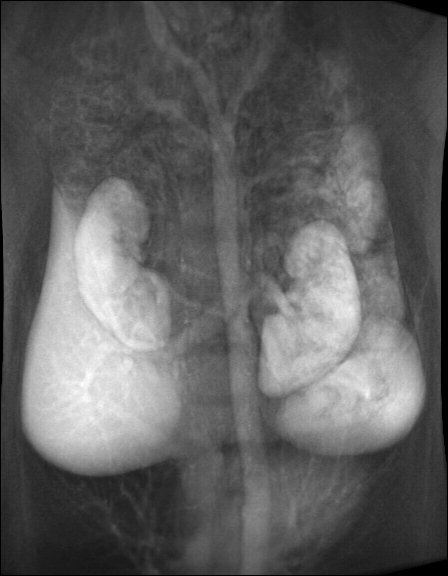
\includegraphics{beaufix_AIP.jpg}
   \end{minipage} \hfill
   \begin{minipage}[c]{.46\linewidth}
      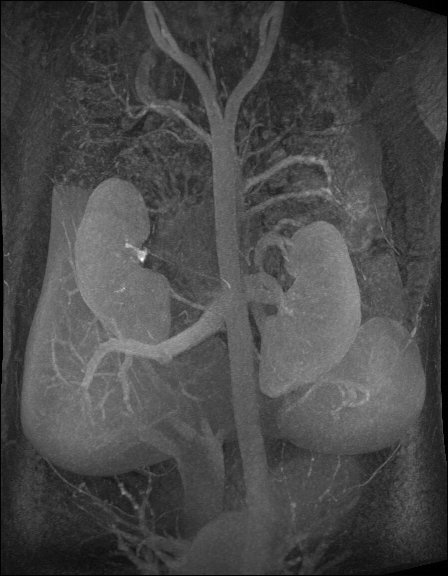
\includegraphics{beaufix_MIP.jpg}
   \end{minipage}
\end{figure}



\end{document}

